\documentclass{beamer}
\mode<presentation>
\usepackage{amsmath}
\usepackage{amssymb}
%\usepackage{advdate}
\usepackage{adjustbox}
\usepackage{subcaption}
\usepackage{enumitem}
\usepackage{multicol}
\usepackage{listings}
\usepackage{url}
\def\UrlBreaks{\do\/\do-}
\usetheme{Boadilla}
\usecolortheme{lily}
\setbeamertemplate{footline}
{
  \leavevmode%
  \hbox{%
  \begin{beamercolorbox}[wd=\paperwidth,ht=2.25ex,dp=1ex,right]{author in head/foot}%
    \insertframenumber{} / \inserttotalframenumber\hspace*{2ex} 
  \end{beamercolorbox}}%
  \vskip0pt%
}
\setbeamertemplate{navigation symbols}{}

\providecommand{\nCr}[2]{\,^{#1}C_{#2}} % nCr
\providecommand{\nPr}[2]{\,^{#1}P_{#2}} % nPr
\providecommand{\mbf}{\mathbf}
\providecommand{\pr}[1]{\ensuremath{\Pr\left(#1\right)}}
\providecommand{\qfunc}[1]{\ensuremath{Q\left(#1\right)}}
\providecommand{\sbrak}[1]{\ensuremath{{}\left[#1\right]}}
\providecommand{\lsbrak}[1]{\ensuremath{{}\left[#1\right.}}
\providecommand{\rsbrak}[1]{\ensuremath{{}\left.#1\right]}}
\providecommand{\brak}[1]{\ensuremath{\left(#1\right)}}
\providecommand{\lbrak}[1]{\ensuremath{\left(#1\right.}}
\providecommand{\rbrak}[1]{\ensuremath{\left.#1\right)}}
\providecommand{\cbrak}[1]{\ensuremath{\left\{#1\right\}}}
\providecommand{\lcbrak}[1]{\ensuremath{\left\{#1\right.}}
\providecommand{\rcbrak}[1]{\ensuremath{\left.#1\right\}}}
\theoremstyle{remark}
\newtheorem{rem}{Remark}
\newcommand{\sgn}{\mathop{\mathrm{sgn}}}
\providecommand{\abs}[1]{\left\vert#1\right\vert}
\providecommand{\res}[1]{\Res\displaylimits_{#1}} 
\providecommand{\norm}[1]{\lVert#1\rVert}
\providecommand{\mtx}[1]{\mathbf{#1}}
\providecommand{\mean}[1]{E\left[ #1 \right]}
\providecommand{\fourier}{\overset{\mathcal{F}}{ \rightleftharpoons}}
%\providecommand{\hilbert}{\overset{\mathcal{H}}{ \rightleftharpoons}}
\providecommand{\system}{\overset{\mathcal{H}}{ \longleftrightarrow}}
	%\newcommand{\solution}[2]{\textbf{Solution:}{#1}}
%\newcommand{\solution}{\noindent \textbf{Solution: }}
\providecommand{\dec}[2]{\ensuremath{\overset{#1}{\underset{#2}{\gtrless}}}}
\newcommand{\myvec}[1]{\ensuremath{\begin{pmatrix}#1\end{pmatrix}}}
\let\vec\mathbf

\lstset{
%language=C,
frame=single, 
breaklines=true,
columns=fullflexible
}

\numberwithin{equation}{section}

\title{9.4.22}
\author{Prajwal \\ EE24BTECH11051 \\ Dept. of Electrical Eng.,\\IIT Hyderabad.}

\date{\today} 
\begin{document}

\begin{frame}
\titlepage
\end{frame}
\section*{Outline}
\begin{frame}
\tableofcontents
\end{frame}
\section{Problem}
\begin{frame}
\frametitle{Problem Statement}
In a culture, the bacteria count is 1,00,000. The number is increased by $10\%$ in 2 hours. In how many hours will the count reach 2,00,000, if the rate of growth of bacteria is proportional to the number present?
\end{frame}
\section{Solution}
\subsection{Table}
\begin{frame}[fragile]
\frametitle{Table}
    \begin{table}[h!]
        \centering
        \begin{tabular}[12pt]{|c|c|}
     \hline
     {variable} & {description}\\
     \hline
     $N$ & Number of bacteria at any time t\\
     \hline
     $t$ & time in hours\\
     \hline
     $C$ & primary arbitrary constant\\
     \hline
     $C_1$ & secondary arbitrary constant\\
     \hline
     $k$ & proportionality constant\\
     \hline
     $N_0$ & initial Number of bacteria\\
     \hline
     
\end{tabular}

        \caption{Variables Used}
        \end{table}
\end{frame}

%\subsection{Literature}
\subsection{Solution}
\begin{frame}
\frametitle{Solution}
Let N be the number of bacteria at any time t. According to the given problem, Rate of change in number of bacteria can be given as 
\begin{align}
\frac{dN}{dt} \propto N \label{1}
\end{align}
\begin{align}
\frac{dN}{dt} = k \times N \label{2}
\end{align}
Seperating the variables in the equation \eqref{2}, We get 
\begin{align}
\frac{dN}{N}=k \times dt \label{3}
\end{align}
On integrating both sides
\begin{align}
\int \frac{dN}{N}=k\int dt  \label{4} \\
log N = k \times t+C \label{5} \\
N=e^{kt+C} \label{6} \\
N=e^{kt} . e^{C} \label{7} \\
\end{align}
\end{frame}
\begin{frame}
\begin{align}
    N=e^{kt} . C_1 \label{8}
\end{align}
Given, at time t=0,$N_0$=1,00,000 then, from \eqref{8}
\begin{align}
N_0=C_1=1,00,000 \label{9}
\end{align}
number of bacteria can be given as 
\begin{align}
N = N_0 e^{kt} \label{10}
\end{align}
At time t=2,number of bacteria is increased by $10\%$ of 1,00,000 from \eqref{8} \\
\begin{align}
1,10,000 =1,00,000\times e^{kt} \\
1,10,000 =1,00,000 \times e^{k\times 2} \\
1.1 = e^{k\times 2} \\
k = \frac{log (1.1)}{2}
\end{align}
\end{frame}
\begin{frame}
number of bacteria can be given as 
\begin{align}
N = N_0e^{kt} \label{10}
\end{align}
rearranging the variables,
\begin{align}
\frac{1}{k}log \brak{\frac{N}{N_0}} = t\label{10}
\end{align}
for N=2,00,000 time is,
\begin{align}
    t = 14.55 \ \textbf{hours}
\end{align}
\end{frame}
\section{Logic used for programming}
\subsection{Method of finite difference}
\begin{frame}[fragile]
\frametitle{Method of finite differences}
This method is used to find the approximate solution of the given differential equation by using the values of the function at discrete points.  \\
From the defination of derivative of a function 
\begin{align}
\frac{dy}{dx} \approx \frac{y\brak{x+h}-y\brak{x}}{h} \label{11}
\end{align}
by rearranging the terms, we get the function
\begin{align}
y\brak{x+h}=y\brak{x}+h \times \frac{dy}{dx} \\
N\brak{t+h}=N\brak{t}+h \times N \times k
\end{align}
Let \brak{t_0,N_0} be points on the curve,
\begin{align}
t_1=t_0+h \\
N_1=N_0+h \times N \times k
\end{align}
\end{frame}
\begin{frame}[fragile]
    On  generalising the above equations,
\begin{align}
t_{n+1}=t_{n}+h \\
N_{n+1}=N_{n}+h \times N \times k \label{21}
\end{align}
Where h is a very small division (example 0.1),We need iterate this algorithm by taking $N_0=1,00,000$ and $t=0$, till $t_n=15$. Then we get the number of bacteria  after 15 hours.
If we plot all the points $(t,N)$, we get the function N varying with t, i.e N vs T graph. \\
\end{frame}
\subsection{Solution of differential equation using the Z-Transform}
\begin{frame}[fragile]
\frametitle{Solution of differential equation using the Z-Transform}
By using the z-transform method we can convert the differential equation into a linear equation in Z-domain,after finding the solution in z-domin,inverse of it is the solution of the given differential equation. \\
The differential equation for this question is,
\begin{align}
\frac{dN}{dt}=N \times k
\end{align}
from \eqref{21}, \\
\begin{align}
N_{n+1}=N_{n}+h \times N \times k \\
N_{n+1}=N_{n}(1+h \times k)
\end{align}
Applying Z-tranform on both sides,We get,
\begin{align}
Z\brak{N_{n+1}}=Z\brak{N_{n}(1+h \times k)} \\
Z(N_n+1)=(1+h\times k)Z(N_n)
\end{align}
\end{frame}
\begin{frame}[fragile]
Let,
\begin{align}
Z\brak{N_n}=N\brak{z}
\end{align}
Then,
\begin{align}
Z\brak{N_{n+1}}=zN(z)-zN_0
\end{align}
Now,
\begin{align}
zN(z)-zN_0 = N(z)(1+h\times k) \\
N(z) \sbrak{z-\brak{1+h \times k}} = zN_0 \\
\end{align}
\begin{align}
N(z) = N_0 \sbrak{\frac{z}{z-\brak{1+h \times k}}}
\end{align}
\end{frame}
\begin{frame}[fragile]
    By inversing, we get 
\begin{align}
N_n = N_0 \times \brak{1+h \times k}^n
\end{align}
We know that,
\begin{align}
1+h \times k \approx e^{h \times k}
\end{align}
then,
\begin{align}
N_n = N_0 \brak{e^{h\times k}}^n \\
N_n = N_o e^{n\times k \times h}
\end{align}
As h is the small division of time and n are the total no.of divisions, nh turns to be t at that point,Then
\begin{align}
N\brak{t}=N_0e^{kt}
\end{align}
\end{frame}
\section{Codes}
\subsection{C code}
\begin{frame}[fragile]
\frametitle{C code}
    \begin{lstlisting}
#include <stdio.h>
#include<math.h>
void fun(double n,double t,double h,double *x,double *y){
  n=100000;
  t=0;
  h=0.1;
   double k = log(11.0 / 10.0) * 0.5;
  for(int i=0;i<100;i++){
    x[i]=t;
    y[i]=n;
    n = n * (1 + h * k); 
    t=t+h;
  }
}
\end{lstlisting}
\end{frame}
\subsection{Pyhton code}
\begin{frame}[fragile]
    \begin{lstlisting}
        import numpy as np
import matplotlib.pyplot as plt
import ctypes

# Load the shared object (.so) file
# Replace './code.so' with the actual path to your .so file
c_lib = ctypes.CDLL('./code.so')

# Define the numerical function signature
# void fun(double n, double t, double h, double *x, double *y, int steps)
c_lib.fun.argtypes = [
    ctypes.c_double,  # Initial population
    ctypes.c_double,  # Start time
    ctypes.c_double,  # Step size
    ctypes.POINTER(ctypes.c_double),  # Array for x (time)
    ctypes.POINTER(ctypes.c_double),  # Array for y (population)
    ctypes.c_int      # Number of steps
]
    \end{lstlisting}
\end{frame}
\begin{frame}[fragile]
\begin{lstlisting}
    k=np.log(11/10)*(0.5)
# Wrapper for the C function
def numerical_solution_from_so():
    # Time step and total steps
    h = 0.1
    t_max = 14.55  # Calculate number of steps

    # Allocate arrays for t (x) and n (y)
    x = (ctypes.c_double * 100)()
    y = (ctypes.c_double * 100)()
    
    # Initial values
    n = ctypes.c_double(100000)
    t = ctypes.c_double(0)
    
    # Call the C function
    c_lib.fun(n, t, ctypes.c_double(h), x, y, ctypes.c_int(100))
    \end{lstlisting}
\end{frame}
\begin{frame}[fragile]
    \begin{lstlisting}
            # Convert the results to numpy arrays
    return np.array(x[:100]), np.array(y[:100])

# Analytical expression N = 100000 * e^(t*k)
def analytical_solution(t):
    return 100000 * np.exp(t*k)

# Z-transform method (discretized version)
def z_transform_solution():
    h = 0.1
    n = 100000
    t = 0
    t_max = 14.55
    x = []
    z = []
    while t <= t_max:  # Iterate up to 14.55 hours
        x.append(t)
        z.append(n)
    \end{lstlisting}
\end{frame}
\begin{frame}[fragile]
    \begin{lstlisting}
                n = n * (1 + h*k)  # Z-transform equivalent
        t = t + h
    return np.array(x), np.array(z)

# Time values for analytical solution
t_values = np.linspace(0, 14.55, 150)

# Get solutions
x_numerical, y_numerical = numerical_solution_from_so()
print(y_numerical)
x_z, z_values = z_transform_solution()
analytical_values = analytical_solution(t_values)
    \end{lstlisting}
\end{frame}
\begin{frame}[fragile]
    \begin{lstlisting}
        # Plotting
plt.figure(figsize=(10, 6))
plt.plot(t_values, analytical_values / 1e5, label='Theory', color='black', linestyle='-')  # Black line for theory
plt.scatter(x_numerical, y_numerical / 1e5, label='Sim1', color='red')  # Red dots for sim1
plt.plot(x_z, z_values / 1e5, label='Sim2', color='blue', linestyle='--')  # Blue dashed line for sim2
plt.xlabel('Time (t) [hours]')
plt.ylabel('N (in lakhs)')
plt.legend()
plt.grid()
plt.title('Bacteria Growth from $t=0$ to $t=14.55$ hours')
plt.savefig('plot.png')  # Save the figure as PNG
plt.show()
    \end{lstlisting}
\end{frame}
\section{Plot}
\subsection{Graph}
\begin{frame}[fragile]
\frametitle{Plot}
    \begin{figure}[htbp] % Positioning options: here, top, bottom, page
    \centering
    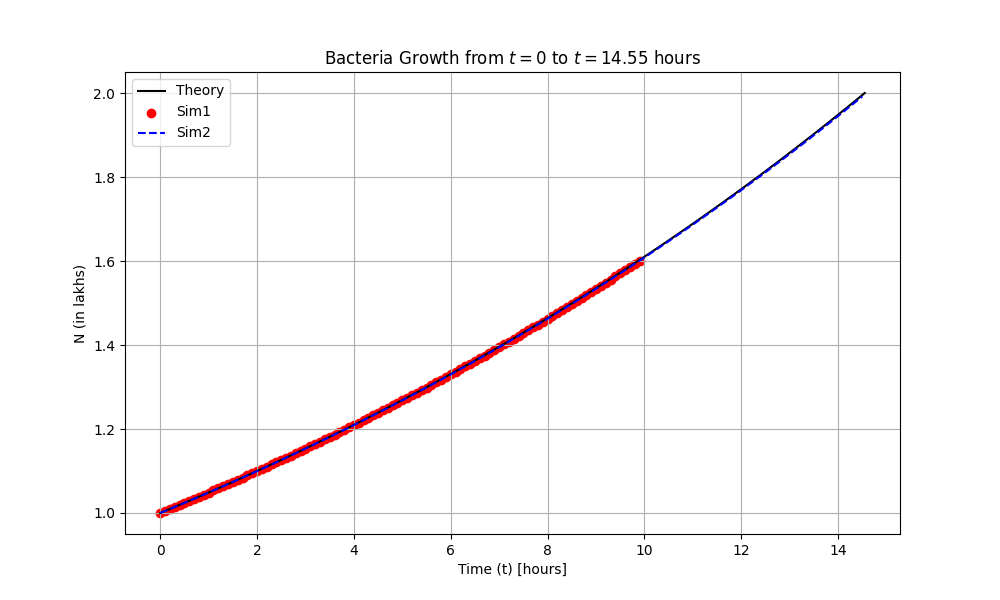
\includegraphics[width=\textwidth]{figs/plot.png} % Replace "filename" with your image file
    \caption{Number of bacteria vs time}
\end{figure}
\end{frame}

\end{document}
